In the system there are four different layer web interface layer, wireless connection layer, base station layer and camera layer. Each and every camera has their unique IP address. When the user enters the IP address in the web browser, it will show the login screen. User has to put the valid username and password to get the access. When the user enters the username and password the system will compare the data entered with the data in the database saved in the raspberry pi. The data will be sent wirelessly, which is received by the black box connected to the raspberry pi through Ethernet connection. If the data entered is valid then the system will take the user to screen, which contains the live streaming video and arrow keys button, which user can use to control the movement of the camera. If the user wants to move the camera and press button, then the message will be sent and which be received by the black box then sent to the raspberry pi. The raspberry pi will control the movement of the stepper. To control the movement of the stepper motors, stepper motor driver has been installed in raspberry pi. At the same time base station will be set up on the remote location which will be main source of the power for the camera layer. As soon as user login, user can start viewing the live streaming video, which user does not have to request. The zoom in and zoom out functionality works in the same way as moving the camera module.


\begin{figure}[h!]
	\centering
 	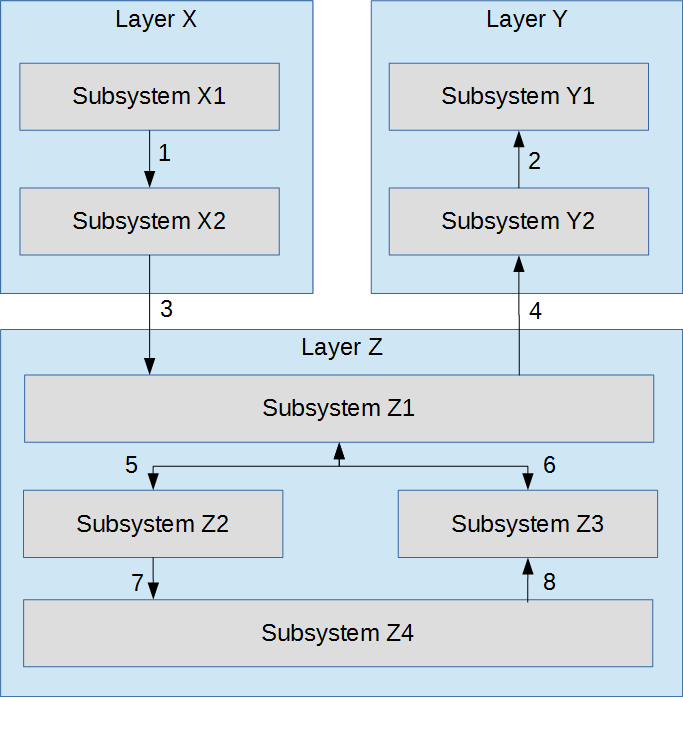
\includegraphics[width=\textwidth]{images/data_flow}
 \caption{A simple data flow diagram}
\end{figure}
